\documentclass[graphics]{beamer}
\usepackage{xcolor}
\usepackage{graphicx}
\usepackage{verbatim}
\usepackage{wrapfig}
\usepackage{tabularx}
\usepackage{multirow}
\usepackage{amssymb}
\usepackage{pifont}
\usepackage{tikz}
\def\Checkmark{\tikz\fill[scale=0.2](0,.35) -- (.25,0) -- (1,.7) -- (.25,.15) -- cycle;} 

\useoutertheme{shadow}
%\usecolortheme{orchid}
\usecolortheme{seahorse}
\newcommand{\cmark}{\text{\ding{51}}}
%\newcommand*{\GtrSim}{\smallrel\gtrsim}

% math commands
\newcommand{\be}{\begin{eqnarray}}
\newcommand{\ee}{\end{eqnarray}}
\newcommand{\beq}{\begin{equation}}
\newcommand{\eeq}{\end{equation}}
\def\simless{\mathbin{\lower 3pt\hbox
      {$\rlap{\raise 5pt\hbox{$\char'074$}}\mathchar"7218$}}}
\def\simgreat{\mathbin{\lower 3pt\hbox
      {$\rlap{\raise 5pt\hbox{$\char'076$}}\mathchar"7218$}}} %> or of order

% variables

\def\toonscale{0.45}
\def\mboxy#1{\mbox{\small #1}}

\defbeamertemplate*{title page}{customized}[1][]
{
  \usebeamerfont{title}\inserttitle\par
  \usebeamerfont{subtitle}\usebeamercolor[fg]{subtitle}\insertsubtitle\par
  \bigskip
  \usebeamerfont{author}\insertauthor\par
  \usebeamerfont{institute}\insertinstitute\par
  \usebeamerfont{date}\insertdate\par
  \usebeamercolor[fg]{titlegraphic}\inserttitlegraphic
}
\begin{comment}
\AtBeginSection[]{
  \frame{
    \frametitle{Outline}
    \tableofcontents[currentsection]
  }
}
\end{comment}


\title{\textcolor{red}{Scintillometry}}
%\subtitle{}
\author[U. Pen]{{
{ 
\textcolor{green}{\small Ue-Li Pen}
}, 
\textcolor{red}{\small Toronto Scintillometry Collaboration} 
}
\\[8mm] 
\textcolor{black}{\small photo: Andre Renard}
}
\date{\textcolor{blue}{March 19, 2019}}



\begin{document}


%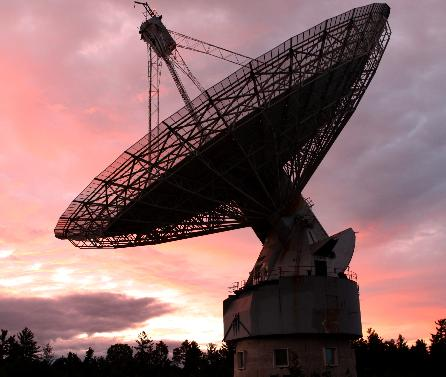
\includegraphics[width=4.4in]{Figures/IMG-7749-ARO-crop.JPG}

\frame{
\vspace{-0.5in}
\begin{center}  
%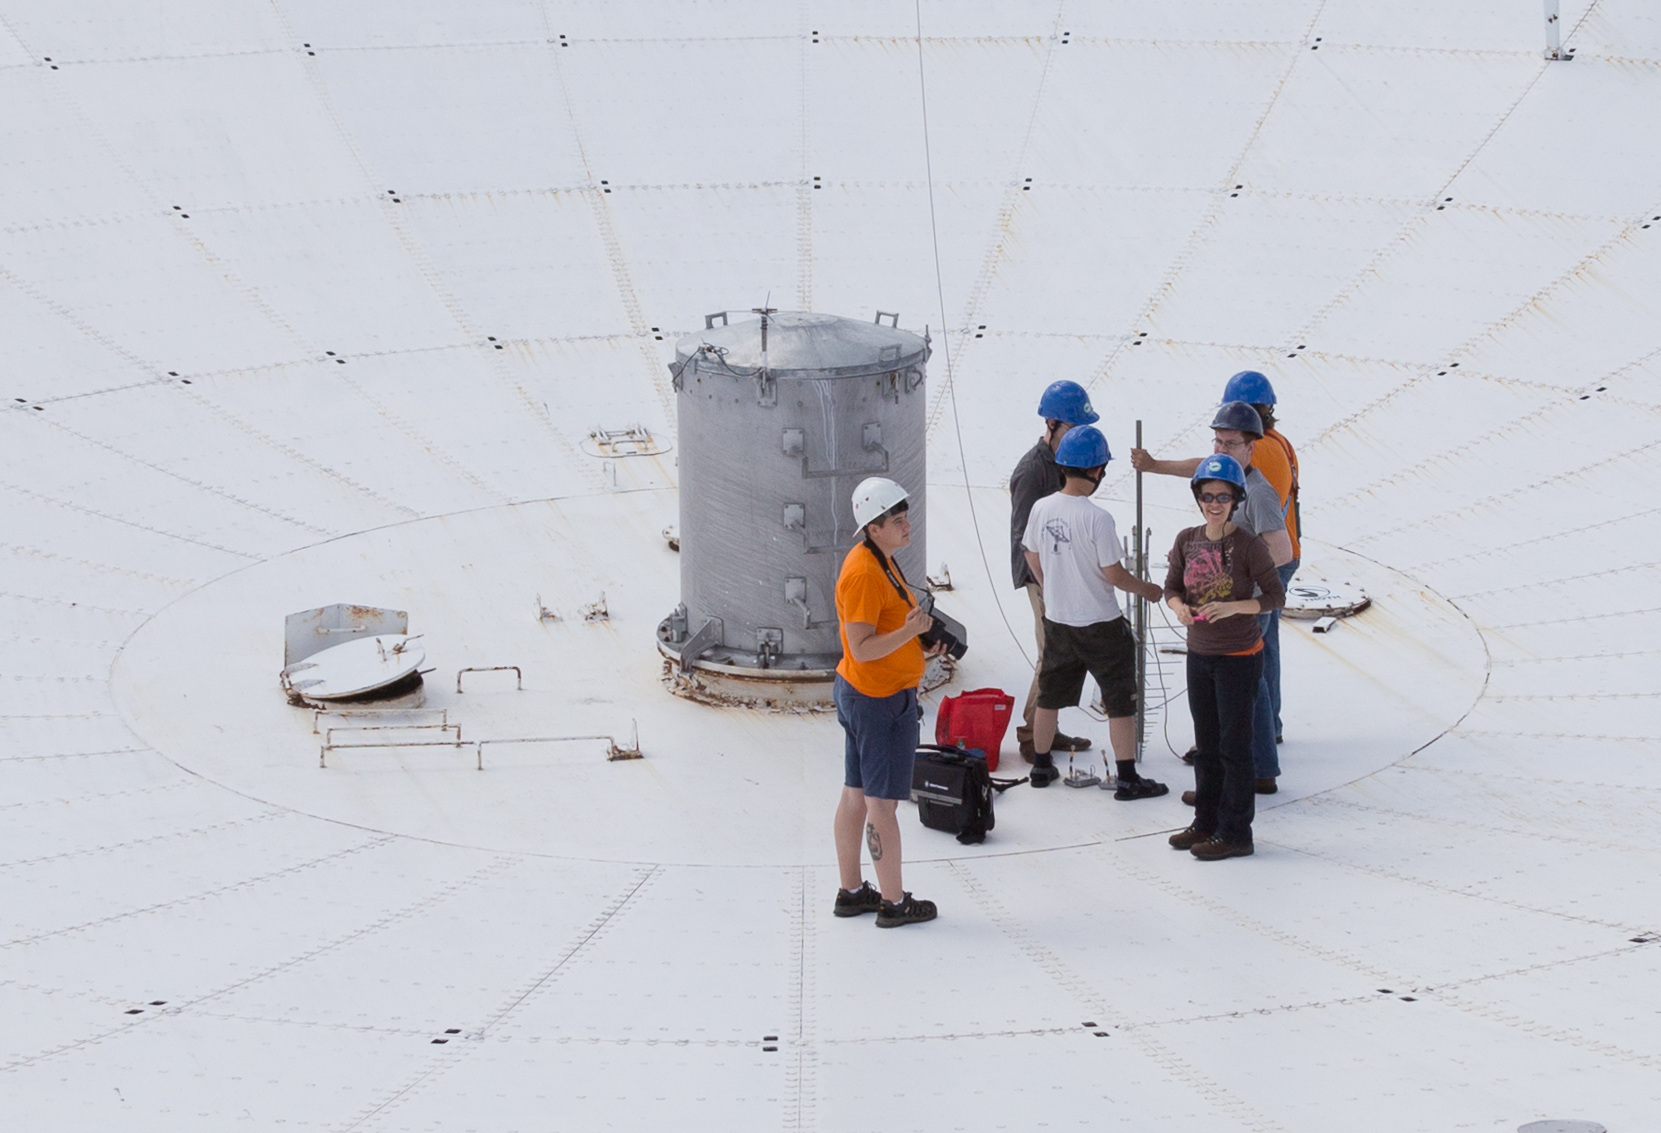
\includegraphics[width=4.4in]{Figures/IMG-0438-by-Andre-cropped.jpg}
\end{center}
\begin{picture}(320,250)
\put(-50,60){
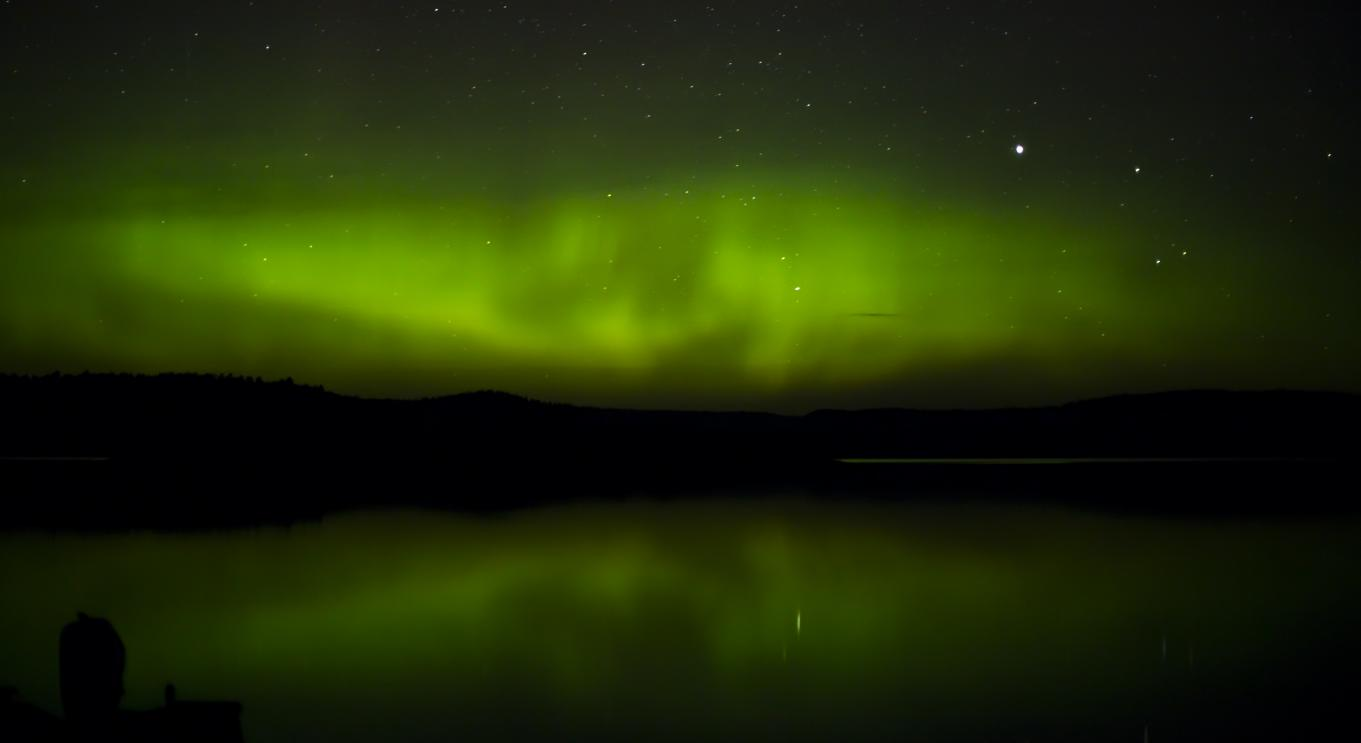
\includegraphics[width=5.5in]{Figures/traverse-aurora.jpg}}
\end{picture}
\vspace{-4in}
\\
image credit: Andre Recnik
\\
\vspace{1in}
\titlepage
}


%\section*{Introduction}
\section{Introduction}

\begin{comment}
  \subsection{Outline}

  \frame{
    \frametitle{Outline}
    \tableofcontents
  }
\end{comment}

  \frame{
    \frametitle{Overview}
    \begin{itemize}
      \item Exploiting natural lenses
      \item potentially precision pulsar distances, precise PTA GW localization
      \item pico-arcsecond astrometry 
      \item FRB/pulsar emission
      \item nature of lenses
      \item baseband data, VLBI
      \item unique opportunity for GMRT
    \end{itemize}
    \vspace{-1in}\hspace{2.5in}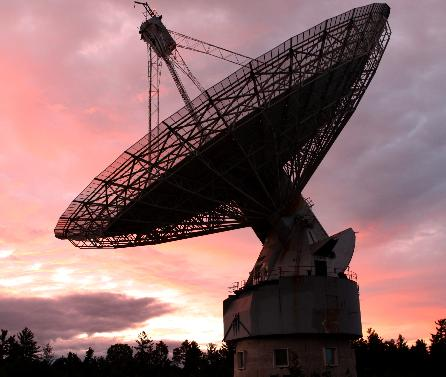
\includegraphics[width=0.5\textwidth]{Figures/IMG-7749-ARO-crop.JPG}
  }

  \frame{
    \frametitle{Natural Lenses}
\hspace{-0.2in}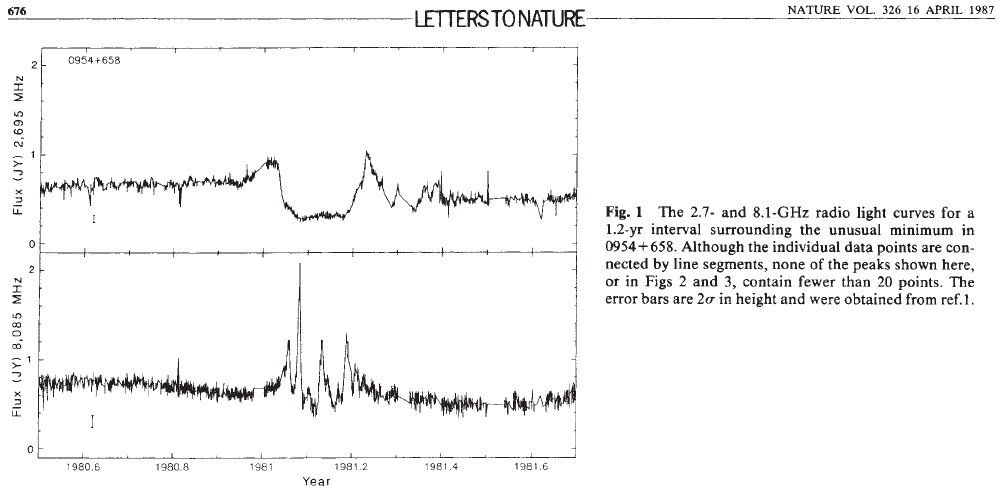
\includegraphics[width=1.1\textwidth]{Figures/fiedler-fig.png}

Fiedler et al 1987
  }
  \frame{
    \frametitle{Natural Lenses}
    \begin{itemize}
      \item Fiedler 1987++: chromatic radio flux variations
      \item evidence for localized ISM lenses: not volume filling
      \item AU transverse scale: if isotropic, requires $n_e\sim 10^3$cm$^{-3}$
      \item ISM explosions, or exotically confined
      \item exploding dark matter, quark nuggets, superconducting
        cosmic strings
      \item hints from pulsar inverted parabolic arclets
      \item lenses elongated, perhaps also along line of sight!
    \end{itemize}
  }

 \frame{
    \frametitle{Sheets}
\hspace{-0.2in}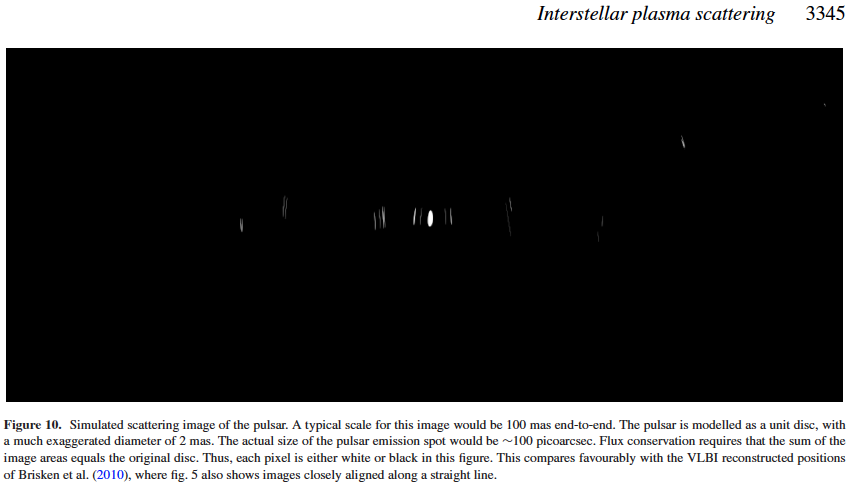
\includegraphics[width=1.05\textwidth]{Figures/lens.png}

Pen and Levin 2014
  }
 \frame{
    \frametitle{Secondary Spectra}
\vspace{-0.75in}
\hspace{0.5in}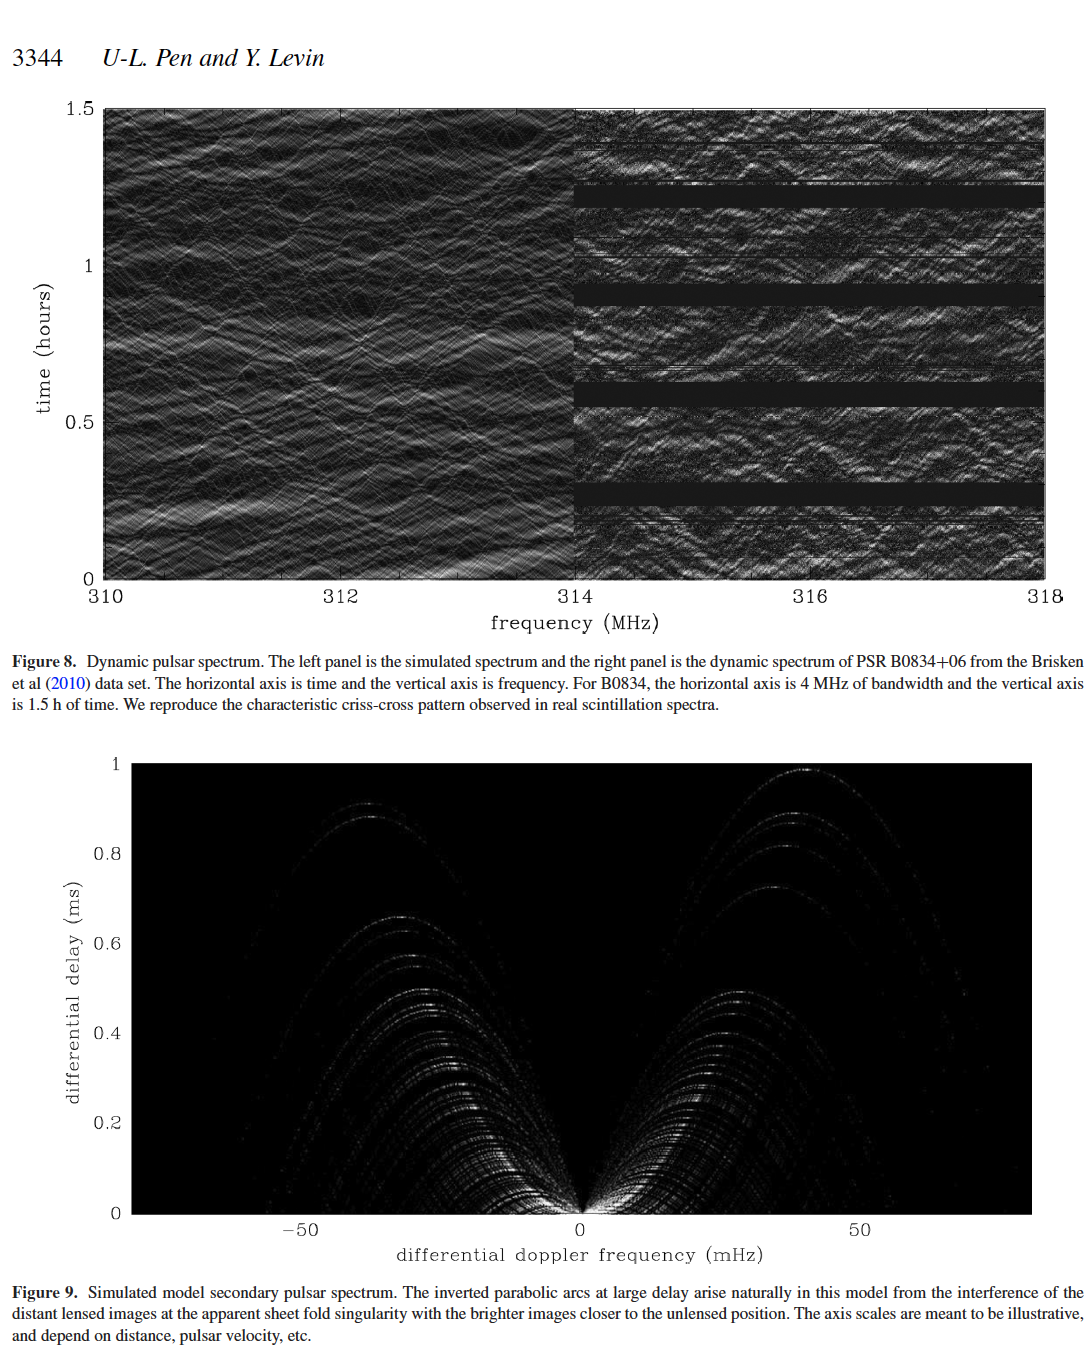
\includegraphics[width=0.7\textwidth]{Figures/dynamic-SS.png}
  }

  \frame{
    \frametitle{Scintillometry}
PSR B0834+06: 

$D_S=620$pc, 

$D_L=389/415$pc

Sheet cusp caustic?

{\tiny Brisken+2010, Liu+2016, Simard+2018}
\begin{picture}(320,250)
\put(110,90){
%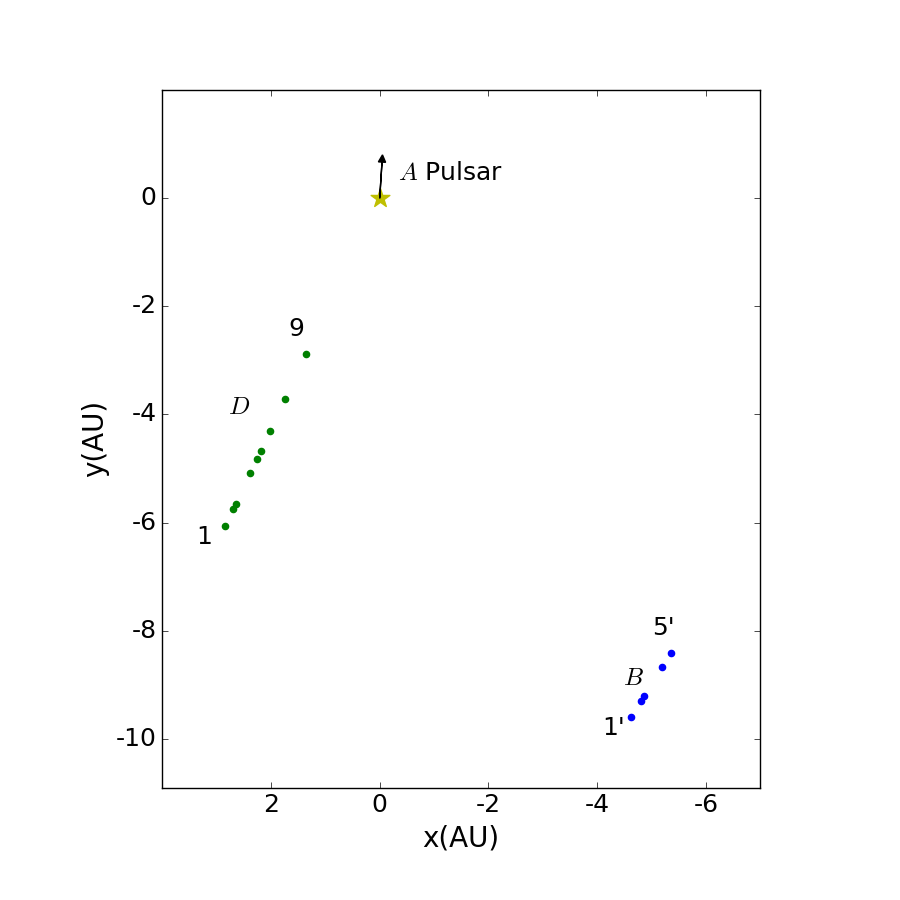
\includegraphics[width=0.7\textwidth]{Figures/Fig7_without_lines_5.png} 
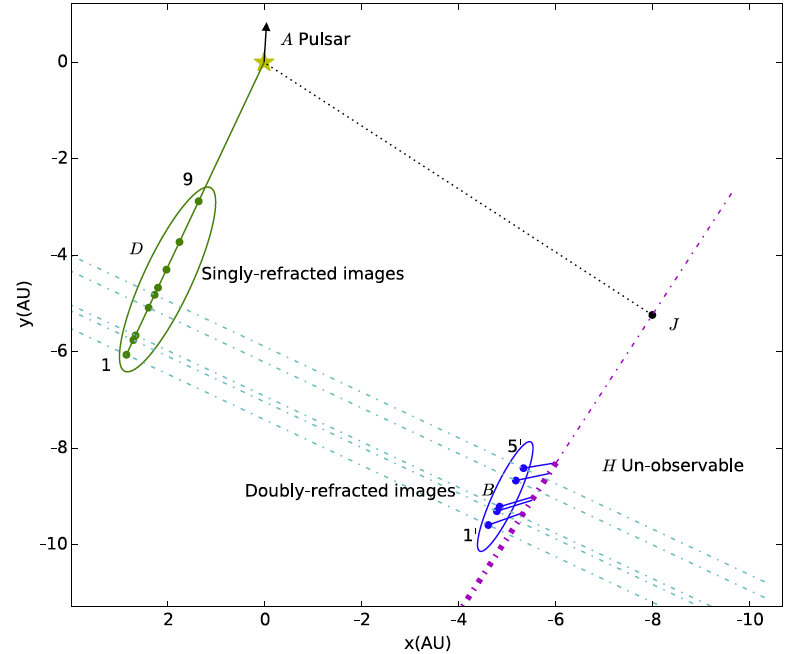
\includegraphics[width=0.7\textwidth]{Figures/liu-lens.png} 

}
\end{picture}
%\vspace{-4in}
\tiny  Brisken+2010, Liu+Pen 2016
  }



\section{Lensing}



  \frame{
    \frametitle{Grazing incidence}
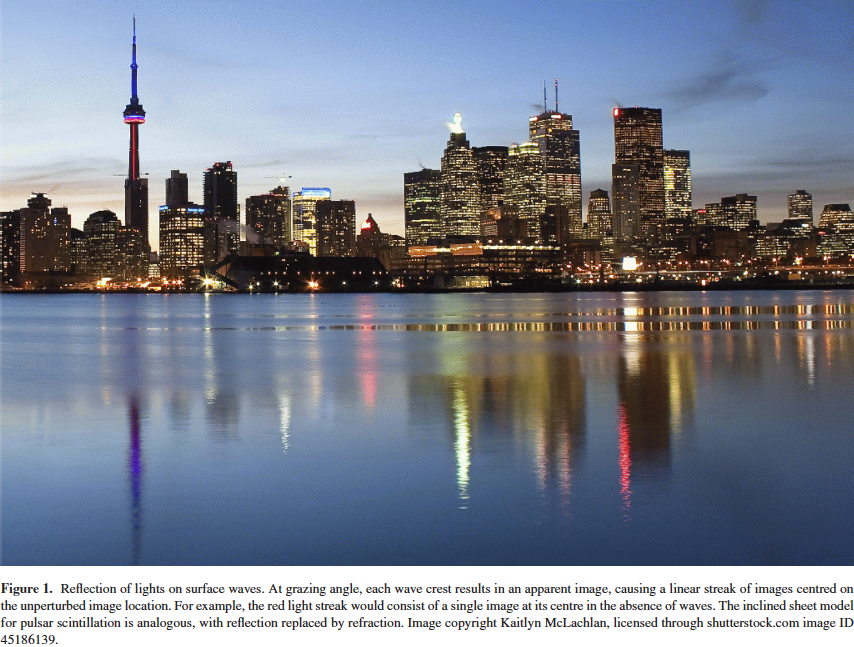
\includegraphics[width=0.9\textwidth]{Figures/toronto.png}
  }


  }
  \frame{
    \frametitle{Applications}
    \begin{itemize}
      \item cosmic telescope: picoarcsecond astrometry of magnetospheres
      \item measured 1km motion of PSR B0834+06 emission, initial results for crab
      \item potential for precision distances to pulsars, increased
        PTA sensitivity, accurate GW localization.
    \item Masui+ 2015, FRB110523: lensing of scattering tail by milky
      way localizes scattering screen to host
      galaxy, rules out IGM scattering
    \item  repeating FRB: potential to discriminate AGN from nebula
    \end{itemize}
  }

  \frame{
    \frametitle{Pulsars}
    \begin{itemize}
    \item plasma microscopes: B1957+20 (see talk by Dongzi)
    \item map distances to invididual screens (see talk by Viswesh)
     \item distances and inclinations to binary pulars: masses, sizes
       (inertia), distances
    \end{itemize}


\vspace{-0.3in}\hspace{1.8in} 
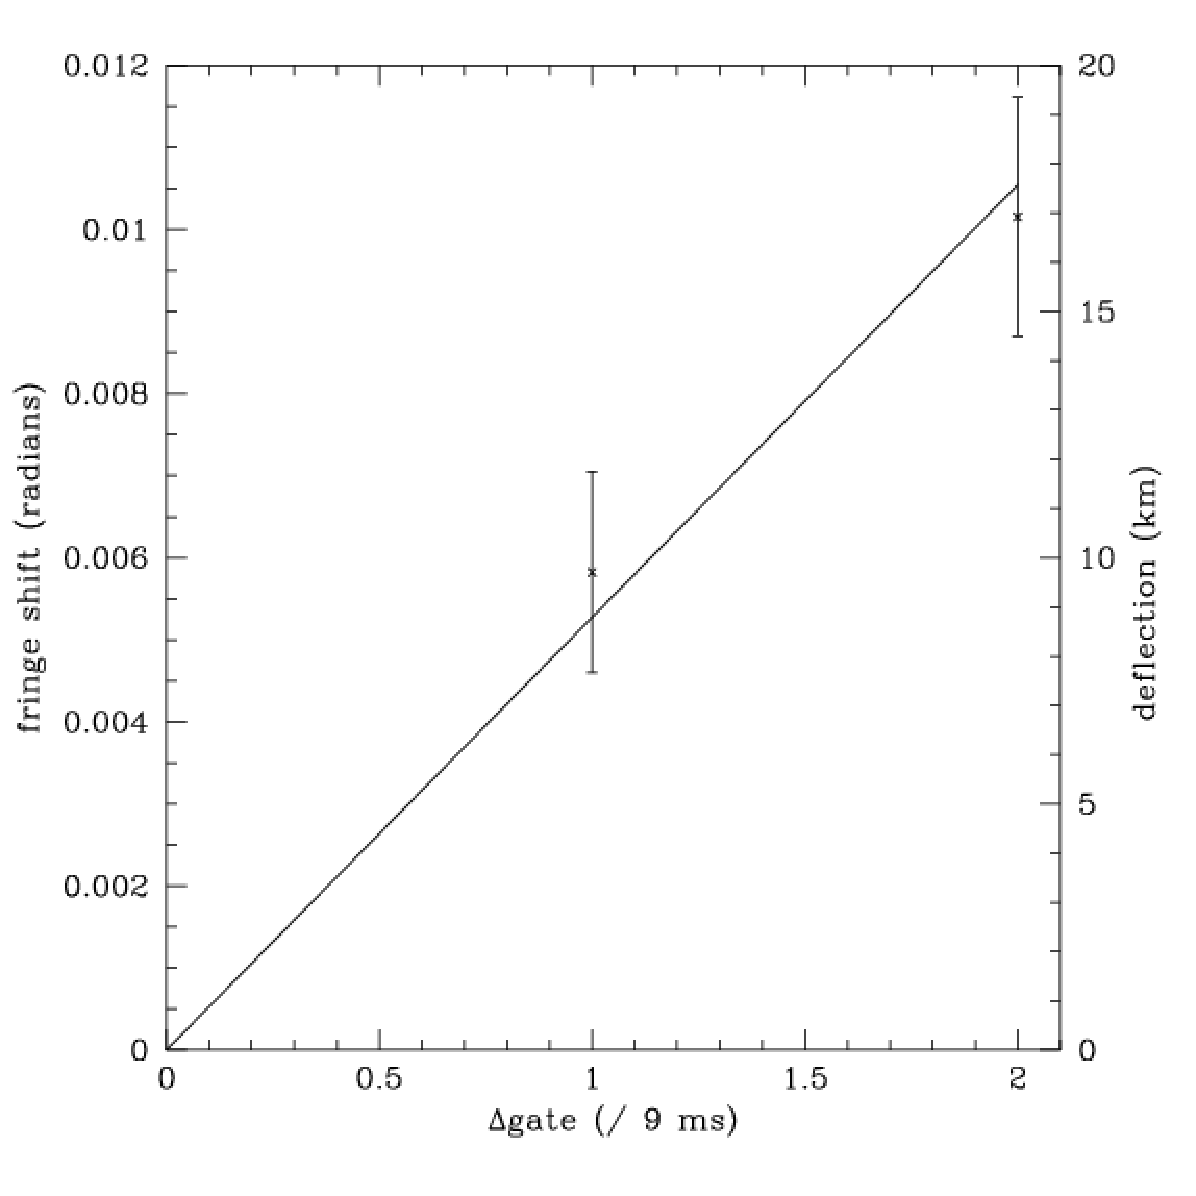
\includegraphics[width=0.4\textwidth]{Figures/allgate.pdf}
\vspace{0.5in}
\tiny Pen+ 2014
.
  }




  \frame{
    \frametitle{Discussion}
    \begin{itemize}
      \item ISM lenses: probed by compact radio sources at high frequencies
      \item pulsars are low frequencies
      \item ISM contains localized, 1-D, strong lensing screens
      \item Pulsars/FRB: unique source of coherent radiation
      \item Use ISM to map source structure
    \end{itemize}
  }


  \frame{
    \frametitle{Conclusion}
    \begin{itemize}
    \item new picture of ISM lensing by small number of inclined sheets
    \item VLBI for screen distances, initial results (incl uGMRT, see
      Viswesh talk)
    \item new analysis techniques needed: coherent imaging, phase retrieval.
    \item unique window on ISM
    \item potential to use scintillometry for precision pulsar
        distances, orbits, masses, improved PTA, emission structures,
        FRB, magnetic fields
    \end{itemize}
  }

\end{document}
